\documentclass[12pt,letterpaper]{exam}
\usepackage[lmargin=1in,rmargin=1in,tmargin=1in,bmargin=1in]{geometry}
\usepackage{../style/exams}

% -------------------
% Course & Exam Information
% -------------------
\newcommand{\course}{MATH 115: Final Exam}
\newcommand{\term}{Fall --- 2024}
\newcommand{\examdate}{12/11/2024}
\newcommand{\timelimit}{150 Minutes}

\setbool{hideans}{false} % Student: True; Instructor: False

\usepackage{polynom}
\usepackage{multicol}
\newenvironment{2enumerate}{%
\begin{enumerate}[(a)]
\begin{multicols}{2}
}{%
\end{multicols}
\end{enumerate}
}

% -------------------
% Content
% -------------------
\begin{document}

\examtitle
\instructions{Write your name on the appropriate line on the exam cover sheet. This exam contains \numpages\ pages (including this cover page) and \numquestions\ questions. Check that you have every page of the exam. Answer the questions in the spaces provided on the question sheets. Be sure to answer every part of each question and show all your work. If you run out of room for an answer, continue on the back of the page --- being sure to indicate the problem number.} 
\scores
\bottomline
\newpage

% Poem
\phantom{.} \vfill
	\begin{table}[h]
	\centering
	\begin{tabular}{l}
	{\itshape 'Twas the night before Christmas, up at the Pole,} \\
	{\itshape Santa was frazzled---he'd lost all control!} \\
	{\itshape The reindeer were restless, the sleight off its track,} \\
	{\itshape And the toy distribution? A logistical smack!} \\
	\\
	{\itshape Santa scratched his beard, eyes weary and red,} \\
	{\itshape ``The math here is tricky. I'm in over my head!} \\
	{\itshape The children are waiting, and I need to take flight.} \\
	{\itshape I need a Precalculus wizard to save Christmas tonight!''}
	\end{tabular}
	\end{table}
\phantom{.} \vfill 

% -------------------
% Questions
% -------------------
\begin{questions}

% Question 1
\newpage
\question[10] {\itshape Santa's lost in the sky, the directions aren't right, \par \phantom{(XX) points)} ``Help me compute these angles to save Christmas night!”} \par\vspace{0.3cm}

Below is a blank unit circle. Fill in each blank entry. The outside blank points should be the point on the unit circle. The innermost blank inside the unit circle should be the angle measure in degrees while the outer blank inside the unit circle is the angle measure in radians. 
	\[
	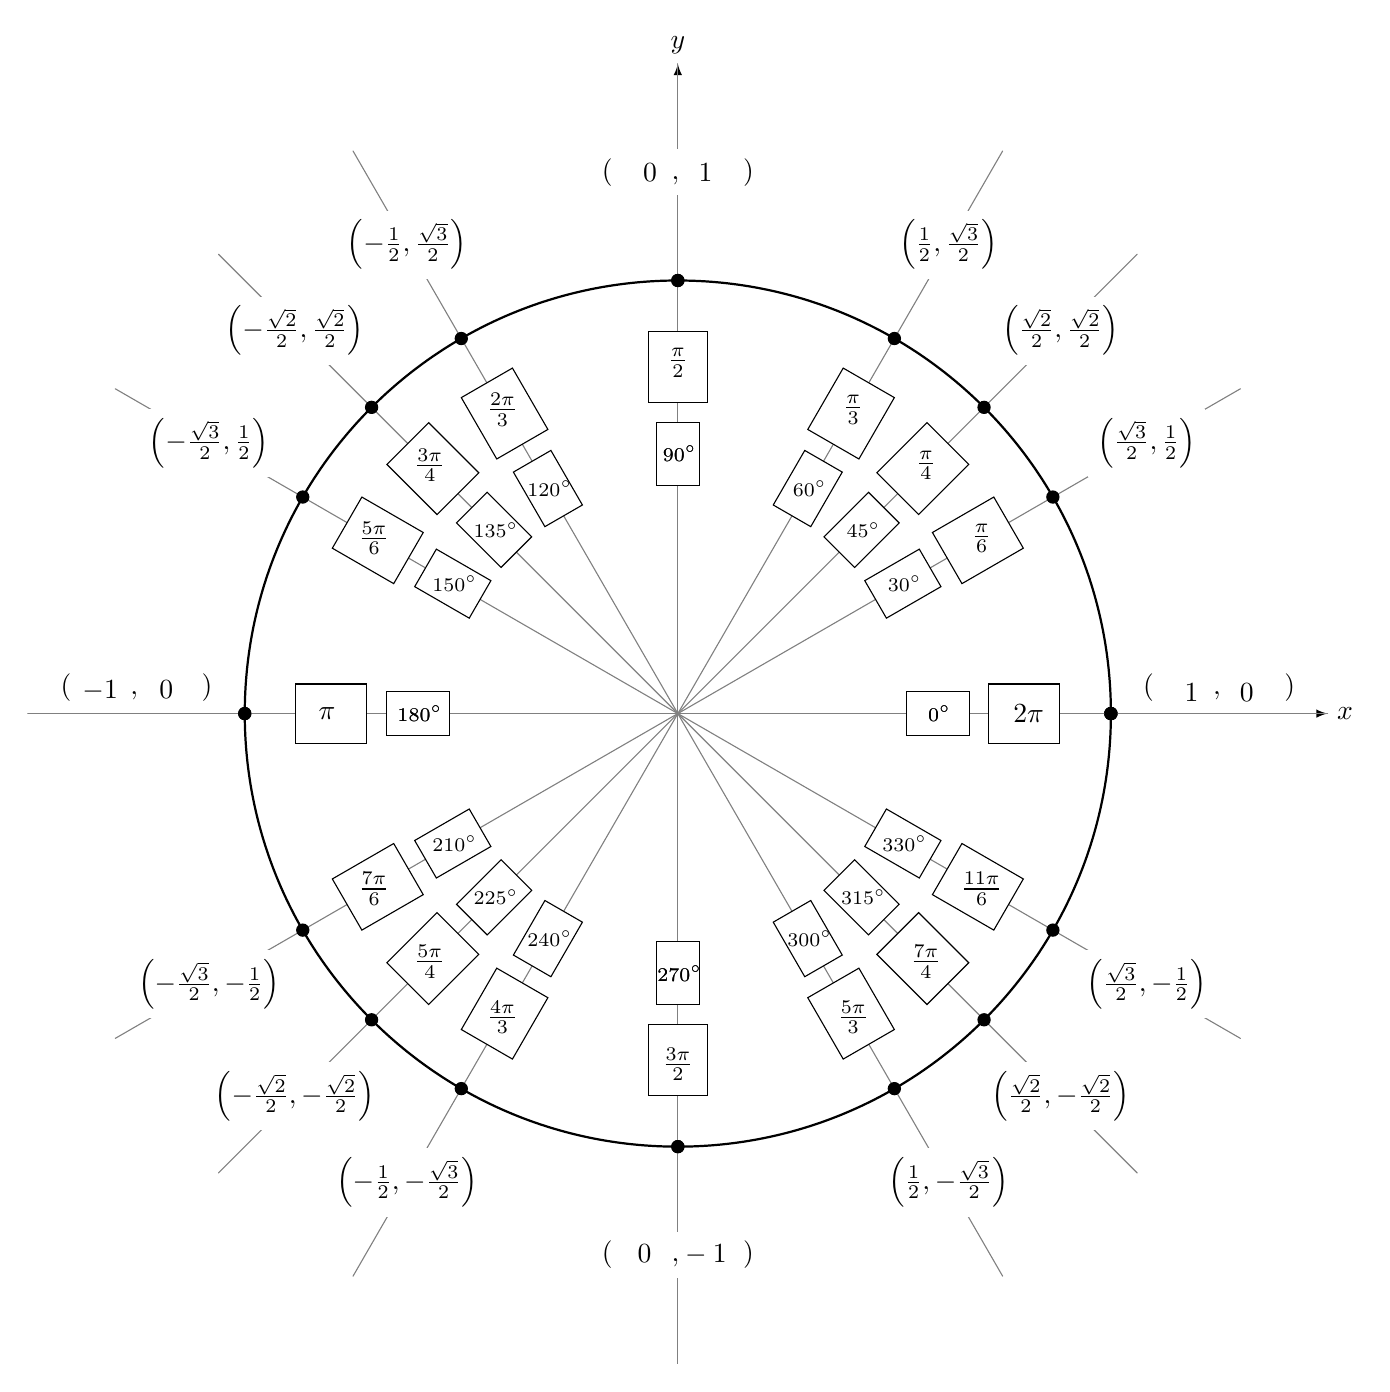
\begin{tikzpicture}[scale=5.5,cap=round,>=latex]

	% Coordinate Axes 
        \draw[->] (-1.5cm ,0cm) -- (1.5cm, 0cm) node[right, fill= white] {$x$};
        \draw[->] (0cm, -1.5cm) -- (0cm, 1.5cm) node[above, fill= white] {$y$};

	% Unit Circle
        \draw[thick] (0cm,0cm) circle(1cm);

	% '30-type' Angles
        \foreach \x in {0,30,...,360} {
                % Line from Center to Point
                \draw[gray] (0cm, 0cm) -- (\x:1.5cm);
                % Dot at Each Points
                \filldraw[black] (\x:1cm) circle(0.4pt);
                % Angles in Degrees
		\draw node[draw, fill= white, shape= rectangle, minimum height= 0.55cm, minimum width= 0.8cm, anchor= center, rotate= \x] at (\x:0.6cm) {};
		% Angle in Radians
		\draw node[draw, fill= white, shape= rectangle, minimum height= 0.75cm, minimum width= 0.9cm, anchor= center, rotate= \x] at (\x:0.8cm) {};
	}
	
	% '45-type' Angles			
	\foreach \x in {0,45,...,360} {
		% Line from Center to Point		
		\draw[gray] (0cm, 0cm) -- (\x:1.5cm);
                % Dot at Each Points			
		\filldraw[black] (\x:1cm) circle(0.4pt);
                % Angles in Degrees
		\draw node[draw, fill= white, shape= rectangle, minimum height= 0.55cm, minimum width= 0.8cm, anchor= center, rotate= \x] at (\x:0.6cm) {};
		% Angle in Radians
		\draw node[draw, fill= white, shape= rectangle, minimum height= 0.75cm, minimum width= 0.9cm, anchor= center, rotate= \x] at (\x:0.8cm) {};
	}
		
	% Horizontal/Vertical Point Placement (Better in this Format)
        \draw (-1.25cm,0cm) node[above=1pt] {$(\hspace{.75cm},\hspace{.75cm})$}
	(1.25cm,0cm)  node[above=1pt] {$(\hspace{.75cm},\hspace{.75cm})$}
	(0cm,-1.25cm) node[fill=white] {$(\hspace{.75cm},\hspace{.75cm})$}
	(0cm,1.25cm)  node[fill=white] {$(\hspace{.75cm},\hspace{.75cm})$};

	% Axes Coordinates
	\draw (-1.27cm,0cm) node[above=1pt] {$-1 \enskip\enskip\enskip 0$}
	(1.25cm,0cm)  node[above=1pt] {$1 \enskip\enskip\enskip 0$}
	(0.01cm,-1.25cm) node[] {$0 \quad -1$}
	(0cm,1.25cm)  node[] {$0 \enskip\enskip\enskip 1$};
	
	% Remainder of Coordinates
	\foreach \x/\xtext/\y in {
		% Q1
		30/\frac{\sqrt{3}}{2}/\frac{1}{2},
		45/\frac{\sqrt{2}}{2}/\frac{\sqrt{2}}{2},
		60/\frac{1}{2}/\frac{\sqrt{3}}{2},
		% Q2
		150/-\frac{\sqrt{3}}{2}/\frac{1}{2},
		135/-\frac{\sqrt{2}}{2}/\frac{\sqrt{2}}{2},
		120/-\frac{1}{2}/\frac{\sqrt{3}}{2},
		% Q3
		210/-\frac{\sqrt{3}}{2}/-\frac{1}{2},
            	225/-\frac{\sqrt{2}}{2}/-\frac{\sqrt{2}}{2},
		240/-\frac{1}{2}/-\frac{\sqrt{3}}{2},
		% Q4
		330/\frac{\sqrt{3}}{2}/-\frac{1}{2},
		315/\frac{\sqrt{2}}{2}/-\frac{\sqrt{2}}{2},
		300/\frac{1}{2}/-\frac{\sqrt{3}}{2}}
		\draw (\x:1.25cm) node[fill=white] {$\left(\xtext,\y\right)$};
	
	% Label Each Angle in Radians
	\foreach \x/\xtext in {
    		30/\frac{\pi}{6},
    		45/\frac{\pi}{4},
    		60/\frac{\pi}{3},
    		90/\frac{\pi}{2},
    		120/\frac{2\pi}{3},
    		135/\frac{3\pi}{4},
    		150/\frac{5\pi}{6},
    		180/\pi,
    		210/\frac{7\pi}{6},
    		225/\frac{5\pi}{4},
    		240/\frac{4\pi}{3},
    		270/\frac{3\pi}{2},
    		300/\frac{5\pi}{3},
    		315/\frac{7\pi}{4},
    		330/\frac{11\pi}{6},
    		360/2\pi}
		\draw (\x:0.81cm) node[] {$\xtext$};

	% Degree Labels (0, 30, 60, ..., 360)
	\foreach \x in {0,30,...,330} {
		\draw (\x:0.6cm) node[] {\scriptsize \,$\x^\circ$};
	}
	
	% Degree Labels (0, 45, 90, ..., 360) 
	\foreach \x in {0,45,...,315} {
		\draw (\x:0.6cm) node[] {\scriptsize \,$\x^\circ$};
	}	
	\end{tikzpicture}
	\]



% Question 2
\newpage
\question[15] {\itshape Santa's sleigh is in trouble, the tech's gone awry, \par \phantom{(XX points)} ``Help me crunch these numbers, or we'll fall out of the sky!”} \par\vspace{0.3cm}

Find the exact value for each of the following: \par\vspace{0.3cm}
	\begin{2enumerate}
	\item $\log_3 \!\left( \dfrac{1}{27} \right)= -3$ \par\vspace{1.8cm}
	\item $\tan(135^\circ)= -1$ \par\vspace{1.8cm}
	\item $\log_5 \left( \sqrt[4]{5} \right)= \frac{1}{4}$ \par\vspace{1.8cm}
	\item $\cos \!\left( \dfrac{5\pi}{3} \right)= \frac{1}{2}$ \par\vspace{1.8cm}
	\item $\tan^{-1}(`\infty\text{'})= \frac{\pi}{2}$ \par\vspace{1.8cm}
	\item $\log_\pi (1)= 0$ \par\vspace{1.8cm}
	\item $\sin \!\left(-\dfrac{2\pi}{3} \right)= -\frac{\sqrt{3}}{2}$ \par\vspace{1.8cm}
	\item $\log_8 (4)= \frac{2}{3}$ \par\vspace{1.8cm}
	\item $\sec(150^\circ)= -\frac{2}{\sqrt{3}}$ \par\vspace{1.8cm}
	\item $\arcsin(0.5)= \frac{\pi}{6}$ \par\vspace{1.8cm}
	\item $\log_{\sqrt{2}}(4)= 4$ \par\vspace{1.8cm}
	\item $\ln(\sqrt{e^3})= \frac{3}{2}$ \par\vspace{1.8cm}
	\item $\arccos(-1)= \pi$ \par\vspace{1.8cm}
	\item $\csc \!\left( -\dfrac{\pi}{6} \right)= -2$ \par\vspace{1.8cm}
	\item $\log_7(7^{\sqrt{3}})= \sqrt{3}$ \par\vspace{1.8cm}
	\item $5^{\log_5(0.71)}= 0.71$ \par\vspace{1.8cm}
	\end{2enumerate}



% Question 3
\newpage
\question[10] {\itshape Santa's sleigh is unsteady, the flight path's complex, \par \phantom{(XX points)} ``Help me save Christmas---just find me the vertex!''} \par\vspace{0.3cm}

Consider the function $f(x)= x^2 + 8x + 13$.
	\begin{enumerate}[(a)]
	\item Find the vertex form of $f(x)$. \pspace
	
	{\itshape By completing the square, we have\dots
		\[
		f(x)= x^2 + 8x + 13= x^2 + 8x + 4^2 - 4^2 + 13= (x^2 + 8x + 16) + (-16 + 13)= (x + 4)^2 - 3
		\]
	Using the evaluation method, we use the fact that the vertex occurs at $x= -\frac{b}{2a}= -\frac{8}{2(1)}= -\frac{8}{2}= -4$, so that the $y$-coordinate is $f(-4)= (-4)^2 + 8(-4) + 13= 16 - 32 + 13= -3$. But then the vertex form is $a(x - P)^2 + Q$, where $(P, Q)$ is the vertex. Therefore, the vertex form is $f(x)= 1\big(x - (-4) \big)^2 + (-3)= (x + 4)^2 - 3$.
		\[
		\boxed{f(x)= (x + 4)^2 - 3}
		\]
	} 
	
	\item Use (a) to identify the vertex for $f(x)$. \pspace
	
	{\itshape We know the $x$-coordinate of the vertex is the $x$-value that `kills' the square term in vertex form and the $y$-coordinate is what remains. Observe that $x= -4$ `kills' the square term: $(-4 + 4)^2 - 3= 0 - 3= -3$. Therefore, the vertex is $(-4, -3)$. Alternatively, the vertex occurs at $x= -\frac{b}{2a}= -\frac{8}{2(1)}= -\frac{8}{2}= -4$, so that the $y$-coordinate is $f(-4)= (-4)^2 + 8(-4) + 13= 16 - 32 + 13= -3$.
	\[
	\boxed{(-4, -3)}	
	\]
	} \pvspace{1.4cm}
	
	\item Use the previous parts to identify the range of $f(x)$. \pspace
	
	{\itshape Because $a= 1 > 0$, the parabola opens upwards, i.e. is convex or concave up. Therefore, $f(x)$ achieves every $y$-value greater than or equal to the $y$-coordinate of the vertex. Therefore, the range is $[-3, \infty)$. 
		\[
		\boxed{\phantom{2_{2_1}^{2^1}} [-3, \infty)^{\phantom{2^1}}}
		\]
	}
	\end{enumerate}



% Question 4
\newpage
\question[10] {\itshape Santa's puzzled by Rudolph, his math seems unclear, \par \phantom{(XX points)}
``Help me check these divisions—Christmas' end is near!''} \par\vspace{0.3cm}

Showing all your work\dots
	\begin{enumerate}[(a)]
	\item Use synthetic division to find the quotient and remainder when $x^4 - 7x^2 - 6x$ is divided by $x + 2$. \pspace
	
	{\itshape First, we need to write the linear divisor as $x - a$. We have $x + 2= x - 2$. We need to be sure the dividend has a term of each degree less than or equal to its degree, which here is four. So, we write $x^4 - 7x^2 - 6x$ as $x^4 + 0x^3 - 7x^2 - 6x + 0$. We can then set-up the chart and perform the computation: \par
		\begin{table}[h]
		\centering
		\begin{tabular}{rrrrrr}
		\multicolumn{1}{r|}{$-2$} & $1$ & $0$ & $-7$ & $-6$ & $0$ \\ \cline{1-1}
		& & $-2$ & $4$ & $6$ & $0$ \\ \hline
		& $1$ & $-2$ & $-3$ & $0$ & $0$
		\end{tabular}
		\end{table}
	Therefore, the quotient is $x^3 - 2x^2 - 3x$ and the remainder is $0$, i.e. $x^4 - 7x^2 - 6x$ is divisible by $x + 2$.
		\[
		\boxed{
		\begin{gathered}
		\text{Quotient} \colon x^3 - 2x^2 - 3x \\
		\text{Remainder} \colon 0
		\end{gathered}}
		\]
	} \pvspace{1.2cm}
		
	\item Find the quotient and remainder when $3x^4 + 4x^3 - 2x^2 + 10x + 2$ is divided by $x^2 + 2x - 1$.  
	
	{\itshape
		\[
		\polylongdiv{3x^4 + 4x^3 - 2x^2 + 10x + 2}{x^2 + 2x - 1}
		\]
	Therefore, the quotient is $3x^2 - 2x + 5$ and the remainder is $-2x + 7$.
		\[
		\boxed{
		\begin{gathered}
		\text{Quotient} \colon 3x^2 - 2x + 5 \\
		\text{Remainder} \colon -2x + 7
		\end{gathered}
		}
		\]
	}
	\end{enumerate}



% Question 5
\newpage
\question[10] {\itshape Santa’s math seems off, his mind’s in a bind, \par \phantom{(XX points)} ``Check my rational computations---I fear I’m behind!''} \par\vspace{0.3cm}

Consider the following function:
	\[
	f(x)= \dfrac{6(x^2 - 1)}{x^2 + 4x - 5}
	\] \pspace
	
\begin{enumerate}[(a)]
\item Find the domain for $f(x)$. \pspace

{\itshape The denominator cannot be zero. We have\dots
	\[
	\begin{gathered}
	x^2 + 4x - 5= 0 \\
	(x + 5)(x - 1)= 0 \\
	x + 5=0 \text{ or } x - 1= 0 \\
	x= -5 \text{ or } x= 1
	\end{gathered}
	\]
Therefore, the domain is the set of real numbers except $x= -5$ and $x= 1$, i.e. $(-\infty, -5) \cup (-5, -1) \cup (-1, \infty)$.}

\item Find any vertical asymptotes for $f(x)$. \pspace

{\itshape The vertical asymptotes are any places where $f(x)$ and the `reduced' $f(x)$ are not defined. We know that $f(x)$ is not defined at $x= -5$ and $x= 1$. Observe that\dots
	\[
	\dfrac{6(x^2 - 1)}{x^2 + 4x - 5}= \dfrac{6(x - 1)(x + 1)}{(x + 5)(x - 1)}= \dfrac{6(x + 1)}{x + 5}
	\]
This reduced function is not defined at $x= -5$. Therefore, the only vertical asymptote for $f(x)$ is $x= -5$.}

\item Find any horizontal asymptotes for $f(x)$. \vfill

{\itshape We have\dots
	\[
	\lim_{x \to \pm\infty} f(x)= \lim_{x \to \pm \infty}  \dfrac{6(x^2 - 1)}{x^2 + 4x - 5}= \dfrac{6}{1}= 6
	\]
Therefore, the only horizontal asymptote is $y= 5$.
}

\item Find any holes for $f(x)$. \pspace

{\itshape Using (a), we know the domain does not include $x= -5$ and $x= 1$. However, from (b), we know that $x= -5$ is a vertical asymptote. Therefore, the only hole occurs at $x= 1$. Using (b), we see the `reduced' $f(x)$ is $\frac{6(x + 1)}{x + 5}$, whose value at $x= 1$ is $\frac{6(2)}{6}= 2$. Therefore, the only whole for $f(x)$ is $(1, 2)$.}
\end{enumerate}



% Question 6
\newpage
\hfill {\itshape Santa's overwhelmed, his gift list is vast, \hfill \phantom{XXXXXXXXXXX} \par
\hfill ``Help me solve these equations---Christmas won't last!''} \hfill \phantom{.} \par\vspace{0.3cm}

\question[10] Showing all your work, solve the equation $\log_2(x + 3) + \log_2(x + 9)= 4$. \pspace

{\itshape Observe\dots
	\[
	\begin{gathered}
	\log_2(x + 3) + \log_2(x + 9)= 4 \\[0.1cm]
	\log_2 \big( (x + 3)(x + 9) \big)= 4 \\[0.1cm]
	2^{\log_2 ( (x + 3)(x + 9) )}= 2^4 \\[0.1cm]
	(x + 3)(x + 9)= 16 \\[0.1cm]
	x^2 + 12x + 27= 16 \\[0.1cm]
	x^2 + 12x + 11= 0 \\[0.1cm]
	(x + 11)(x + 1)= 0 \\[0.1cm]
	x + 11= 0 \text{ or } x + 1= 0 \\[0.1cm]
	x= -11 \text{ or } x= -1
	\end{gathered}
	\] 
But if $x= -11$, we have $\log_2(x + 3)= \log_2(-11 + 3)= \log_2(-8)$, which is not defined. Therefore, $x= -11$ is an extraneous solution. The only solution is $x= -1$.
	\[
	\boxed{\phantom{2_{2_1}^{2^1}} x= -1 \phantom{2_{2_1}^{2^1}}}
	\]
}


% Question 7
\question[10] Showing all your work, solve the equation $19 - e^{-2x}= 12$. \pspace

	\[
	\begin{gathered}
	19 - e^{-2x}= 12 \\[0.3cm]
	-e^{-2x}= -7 \\[0.3cm]
	e^{-2x}= 7 \\[0.3cm]
	\ln e^{-2x}= \ln(7) \\[0.3cm]
	-2x= \ln(7) \\[0.3cm]
	\boxed{x= \dfrac{\ln(7)}{-2}}
	\end{gathered}
	\] \vfill
 
 

% Question 8
\newpage
\question[10] Showing all your work, solve the equation $\sqrt{2x - 1} + 3= 8$. \pspace
	\[
	\begin{gathered}
	\sqrt{2x - 1} + 3= 8 \\[0.3cm]
	\sqrt{2x - 1}= 5 \\[0.3cm]
	2x - 1= 25 \\[0.3cm]
	2x= 26 \\[0.3cm]
	\boxed{x= 13}
	\end{gathered}
	\] \par\vspace{1.2cm}



% Question 9
\question[10] Showing all your work, find the solutions to $x(x + 2) \geq 8$. \pspace
	\begin{minipage}[b]{0.25\textwidth}
	If $x(x + 2) \geq 8$, then \par $x(x + 2) - 8 \geq 0$. We \par then have\dots
		\[
		\begin{gathered}
		x(x + 2) - 8= 0 \\[0.3cm]
		x^2 + 2x - 8= 0 \\[0.3cm]
		(x + 4)(x - 2)= 0 \\[0.3cm]
		x= -4 \text{ or } x= 2
		\end{gathered}
		\]
	\end{minipage} \hspace{0.5cm} \begin{minipage}[b]{0.3\textwidth}
		\[
		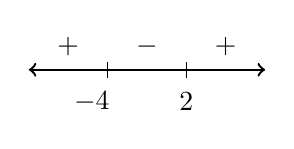
\begin{tikzpicture}
		\draw[line width=0.03cm,<->] (-1.5,0) -- (1.5,0);
		\draw[line width=0.02cm] (-0.5,-0.1) -- (-0.5,0.1);
		\draw[line width=0.02cm] (0.5,-0.1) -- (0.5,0.1);
		\node at (-0.7,-0.4) {$-4$};
		\node at (0.5,-0.4) {$2$};
		\node at (-1,0.3) {$+$};
		\node at (0,0.3) {$-$};
		\node at (1,0.3) {$+$};
		\end{tikzpicture}
		\]
		\[
		\begin{aligned}
		x= -5 &\colon (-5)^2 + 2(-5) - 8= 7 \\[0.1cm]
		x= 0 &\colon 0^2 + 2(0) - 8=-8 \\[0.1cm]
		x= 3 &\colon 3^2 + 2(3) - 8= 7
		\end{aligned}
		\]
	\end{minipage}\hspace{1.4cm}\begin{minipage}[b]{0.3\textwidth}
	Therefore, the solutions \par to the original \par inequality are\dots
		\[
		\boxed{(-\infty, -4] \cup [2, \infty)}
		\]
	\end{minipage} \par\vspace{1.1cm}



% Question 10
\question[10] Showing all your work, solve the equation $\dfrac{3 - x}{x + 3}= x + 1$. \pspace
	\[
	\begin{gathered}
	\dfrac{3 - x}{x + 3}= x + 1 \\[0.1cm]
	3 - x= (x + 3)(x + 1) \\[0.1cm]
	3 - x= x^2 + x + 3x + 3 \\[0.1cm]
	3 - x= x^2 + 4x + 3 \\[0.1cm]
	0= x^2 + 5x \\[0.1cm]
	x(x + 5)= 0 \\[0.1cm]
	x= 0 \text{ or } x + 5= 0 \\[0.1cm]
	\boxed{x= 0 \text{ or } x= -5}
	\end{gathered}
	\]



% Question 11
\newpage
\question[15] {\itshape Santa’s navigation’s out, the sky’s hard to read, \par \phantom{(XX points)} ``Sketch me the path---help me finish this deed!''} \par\vspace{0.3cm}

Consider the function $f(x)= 3\sin(2x - \pi) + 1$.
	\begin{enumerate}[(a)]
	\item Showing all your work, identify the period, amplitude, and phase shift for $f(x)$. \pspace
	
	{\itshape We write $f(x)= 3 \sin(2x - \pi) + 1= 3 \sin \!\big(2 (x + \frac{-\pi}{2}) \big) + 1$. We can then see that\dots
		\[
		\boxed{
		\begin{gathered}
		\text{Period}= \dfrac{2\pi}{2}= \pi \\[0.3cm]
		\text{Amplitude}= 3 \\[0.3cm]
		\text{Phase Shift}= -\frac{\pi}{2}
		\end{gathered}
		}
		\]
	} \pvspace{1.5cm}
	
	\item Use (a) to sketch a graph of $f(x)$. Your plot should contain any $x$- or $y$-intercepts and the location of any maxima or minima. You must graph $f(x)$ over at least one full period. \pspace
	
	{\itshape We can graph $f(x)$ over any period. We will naturally begin at $-\frac{\pi}{2}$---the phase shift. We know the period is $\pi$, which we split into four pieces, $\frac{\pi}{4}$, which we use as our step size. Therefore, the `essential' $x$-values we use for the plot are $-\frac{\pi}{2}$, $-\frac{\pi}{2} + \frac{\pi}{4}= -\frac{\pi}{4}$, $-\frac{\pi}{4} + \frac{\pi}{4}= 0$, $0 + \frac{\pi}{4}= \frac{\pi}{4}$, and $\frac{\pi}{4} + \frac{\pi}{4}= \frac{\pi}{2}$. We know the amplitude is $3$ and the vertical shift is $1$, so that the wave will alternate between $3 + 1= 4$ and $-3 + 1= -2$. This gives the plot below. [The red portion is the plot of the period described and the dotted blue line is the midline..]
		\[
		\fbox{
		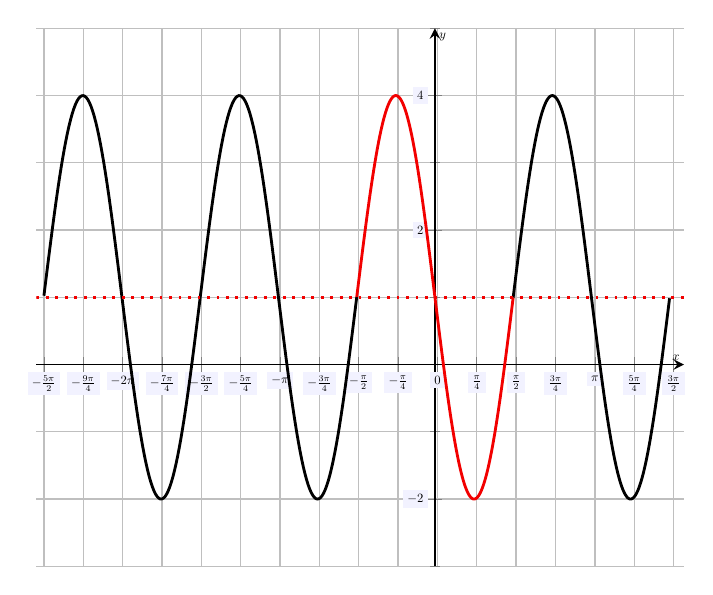
\begin{tikzpicture}[scale=1.2,every node/.style={scale=0.38}]
		\begin{axis}[
		grid = both,
		axis lines=middle,
		ticklabel style={fill=blue!5!white},
		xmin= -8, xmax=5,
		ymin= -3, ymax=5,
		minor x tick num= 0,
		minor y tick num= 1,
		xtick= {-7.85,-7.06,...,7.95},
		xticklabels = {$-\frac{5\pi}{2}$, $-\frac{9\pi}{4}$, $-2\pi$, $-\frac{7\pi}{4}$, $-\frac{3\pi}{2}$, $-\frac{5\pi}{4}$, $-\pi$, $-\frac{3\pi}{4}$, $-\frac{\pi}{2}$, $-\frac{\pi}{4}$, $0$, $\frac{\pi}{4}$, $\frac{\pi}{2}$, $\frac{3\pi}{4}$, $\pi$, $\frac{5\pi}{4}$, $\frac{3\pi}{2}$},
		xlabel=\(x\),ylabel=\(y\)
		]
		\addplot[line width=0.03cm,domain=-7.85:-1.57,samples=200] ({x},{3*sin(deg(2*x - pi)) + 1});
		\addplot[line width=0.03cm,domain=1.57:4.71,samples=200] ({x},{3*sin(deg(2*x - pi)) + 1});
		\addplot[line width=0.03cm,domain=-1.57:1.57,samples=200,red!95!black] ({x},{3*sin(deg(2*x - pi)) + 1});
		\addplot[line width=0.03cm,domain=-8:5,samples=2,red!95!black,dotted] ({x},{1});
		\end{axis}
		\end{tikzpicture}
		}
		\] 
	}
	\end{enumerate}



% Question 12
\newpage
\question[10] {\itshape Santa's exhausted, his mind's in a blur, \par \phantom{(XX points)} ``Help me verify this---I'm not sure what's a blur!''} \par\vspace{0.3cm}

Showing all your work, verify the following trigonometric identity:
	\[
	(\sin \theta + \cos \theta)^2 + (\sin \theta - \cos \theta)^2= 2
	\] \pspace

{\itshape \tsol We begin with the left-hand side and make use of the identity $\sin^2 \theta + \cos^2 \theta= 1$:
	\[
	\begin{gathered}
	(\sin \theta + \cos \theta)^2 + (\sin \theta - \cos \theta)^2 \\[0.3cm]
	(\sin^2 \theta + 2 \sin \theta \cos \theta + \cos^2 \theta) + (\sin^2 \theta - 2 \sin \theta \cos \theta + \cos^2 \theta) \\[0.3cm]
	(1 + 2 \sin \theta \cos \theta) + (1 - 2 \sin \theta \cos \theta) \\[0.3cm]
	(1 + 1) + (2 \sin \theta \cos \theta - 2 \sin \theta \cos \theta) \\[0.3cm]
	2 + 0 \\[0.3cm]
	2
	\end{gathered}
	\]
}



% Question 13
\newpage
\question[20]  {\itshape Christmas almost over, you're nearly clear. \par \phantom{(XX points)} ``Help me find these identities, then we're done for this year.''} \par\vspace{0.3cm}

Complete the following parts:
	\begin{enumerate}[(a)]
	\item Give the double angle identity for $\sin(2\theta)$. \vfill
		\[
		\sin(2\theta)= 2 \sin \theta \cos \theta
		\] \vfill 
	
	\item Give one of the double angle identities for $\cos(2\theta)$. \vfill
		\[
		\cos(2\theta)= 1 - 2\sin^2(\theta)= 2\cos^2(\theta) - 1= \cos^2 \theta - \sin^2 \theta
		\] \vfill 
	
	\item Give the identity for $\cos(A \pm B)$. \vfill
		\[
		\cos(A \pm B)= \cos A \cos B \mp \sin A \sin B
		\] \vfill 
	
	\item Give the half-angle identity for $\sin\!\left( \frac{\theta}{2} \right)$. \vfill
		\[
		\sin\!\left( \frac{\theta}{2} \right)= \pm \sqrt{\dfrac{1 - \cos \theta}{2}}
		\] \vfill 
	
	\item Given $\csc^2 \theta$ in terms of $\cot^2 \theta$. \vfill
		\[
		\csc^2 \theta= 1 + \cot^2 \theta
		\] \vfill 
	\end{enumerate}

\end{questions}


% End Poem
\newpage

\phantom{.} \vfill
	\begin{table}[h]
	\centering
	\begin{tabular}{l}
	{\itshape Santa exclaimed, at the end of Christmas night,} \\
	{\itshape ``Thanks to you, the math's worked out right!} \\
	{\itshape Stay curious, dear student, keeping Mathematics in sight,} \\
	{\itshape And merry Christmas to all, and to all a good night!}
	\end{tabular}
	\end{table}
\phantom{.} \vfill

\end{document}